\documentclass[11pt]{article}
\usepackage[review]{acl}
\usepackage{times}
\usepackage{latexsym}
\usepackage[T1]{fontenc}
\usepackage[utf8]{inputenc}
\usepackage{microtype}
\usepackage{graphicx}
\usepackage{booktabs}
\usepackage{amsmath,amssymb,amsthm}
\usepackage{multirow}
\usepackage{tikz}
\usetikzlibrary{arrows.meta,positioning,fit,backgrounds}
\usepackage{enumitem}

\makeatletter
\ifacl@linenumbers
  \font\aclhvsmall=phvb at 6.5pt
  \renewcommand\linenumberfont{\aclhvsmall\color{lightgray}}
  \setlength{\linenumbersep}{8pt}
\fi
\makeatother

\newtheorem{proposition}{Proposition}
\newcommand{\method}{FinPlan}
\newcommand{\E}{\mathbb{E}}
\newcommand{\Prob}{\mathbb{P}}
\newcommand{\indic}{\mathbf{1}}

\title{\method: Loss-Aware Decision Interfaces for Point-in-Time Financial Evidence}
\author{Anonymous ACL submission}

\begin{document}
\sloppy
\maketitle

\begin{abstract}
Forward-looking financial guidance admits several valid outputs at the filing date: a point answer, a credible set, an abstention, or a decision to wait for a later filing. Existing retrieval-augmented generation and claim-verification systems fix the output mode, decision time, and evidence budget before observing the evidence. We formulate the output contract as a decision problem over a credal state and introduce \method, a loss-aware interface that chooses among answering, adjudicating, abstaining, acquiring evidence, and waiting. \method{} separates a point-in-time evidence model from a decision layer that reads the loss and validation evidence. We release a year-wise company-disjoint benchmark of 273 revenue-guidance claims from SEC filings, with 227 XBRL-verified test claims. On verified labels, the evidence model raises balanced accuracy from .333 to .564 and macro F1 from .220 to .488. On a non-LLM random-forest backbone, a portfolio over fixed adjudication, abstention, and the planner reaches mean oracle regret $-0.037$ with maximum $0.000$, and improves on the best fixed policy under a wide-width penalty by $-0.370$. A pre-specified seed replication preserves the wide-width gain. We instantiate six named baselines from their official source repositories at pinned commits under a shared three-way adapter. Across DeepSeek, GLM 5.3 flash, and a locally served Qwen3-8B, \method{} has the highest balanced accuracy and AUROC; no baseline dominates every metric. On a real earnings-release stream, a sequential portfolio matches the oracle best policy in all 24 cost cells.
\end{abstract}

\section{Introduction}

A company issues quarterly revenue guidance in an 8-K filing. The guidance is a range, and the realized revenue is not known until a later filing. An analyst reading the first filing can return a point forecast, state a credible set of outcomes, decline to answer, or wait for the earnings release. The preferred action depends on the evidence available at the cutoff, the evidence that will arrive, and the cost of each type of error. A narrow range with a reliable current-quarter anchor may justify a point answer. A wide range with no anchor may support only a qualified judgment. A delayed filing may settle the question at a cost in time.

Most financial question answering and claim-verification systems make this choice before seeing the evidence. Retrieval-augmented generation returns a generated answer \citep{lewis2020rag}. Claim verification returns a verdict such as supported or contradicted \citep{zhao2024findver,rangapur2025finfact}. Selective prediction returns an answer or an abstention \citep{chow1970optimum,geifman2017selective}. Adaptive retrieval decides when to retrieve or how many passages to retrieve \citep{jiang2023flare,jeong2024adaptiverag}. These systems improve the evidence or the retrieval policy, but the output contract, the decision time, and the evidence budget remain fixed. A system therefore cannot express a case in which the first evidence supports a credible set, a later filing supports a point answer, and the correct output mode changes between the two moments.

This paper treats the output contract as a decision variable. We represent the state of evidence as a credal set over outcome buckets, define an asymmetric loss over point answers, credible sets, abstentions, evidence acquisition, and delay, and let a planner choose an output action or an evidence action from the current state. The formulation includes fixed-output systems as special cases: a fixed-cutoff RAG system fixes the time and restricts the action set; a verifier fixes the verdict; a selective classifier restricts the output to answer or abstain; a pre-hoc router chooses the mode before evidence arrives. The interface is more general than each of these restrictions and makes the decision time and evidence cost explicit.

We build a benchmark that matches the decision problem. Each claim is a quarterly revenue-guidance statement from a U.S. SEC 8-K filing between 2010 and 2025. The label is whether realized revenue falls below, within, or above the guided range, measured from SEC XBRL. The benchmark uses a year-wise company-disjoint protocol: for each test year, training claims come from other companies and have outcome dates before January 1 of that year. This removes company identity and future outcomes from the training data. The test set has 273 claims from 2022 to 2025, of which 227 have XBRL-verified labels. A rolling-origin extension covers 737 claims from 2015 to 2025.

\paragraph{Contributions.}
Our contributions are fourfold.
\begin{itemize}[leftmargin=*,itemsep=1pt,topsep=2pt]
\item \textbf{Interface.} We formulate point-in-time financial evidence as a credal decision problem with output actions, evidence acquisition, and waiting under an asymmetric loss. Fixed output contracts are special cases rather than assumptions.
\item \textbf{Benchmark.} We release a year-wise, company-disjoint benchmark of 273 revenue-guidance claims and a 737-claim rolling extension, with XBRL label provenance, temporal controls, calibration metrics, selective risk, and a featureless prior control.
\item \textbf{Decision layer.} We introduce a validation-selected portfolio over fixed adjudication, abstention, and a belief-driven planner. On a non-LLM random-forest backbone it matches the oracle best fixed policy in nine of ten loss configurations and improves on it under a wide-width penalty.
\item \textbf{Evidence.} We instantiate six named baselines from their official source repositories at pinned commits under a shared task adapter. Across DeepSeek, GLM 5.3 flash, and a locally served Qwen3-8B, \method{} has the highest balanced accuracy and AUROC, while individual baselines can lead on plain accuracy, selective accuracy, or AURC. On a real earnings-release stream, a sequential portfolio matches the oracle best policy in all 24 cost cells.
\end{itemize}

The benchmark is decision-level. It isolates the output interface and the value of evidence timing; it does not evaluate a long-form reader or a production investment workflow.

\section{Related Work}

\paragraph{Retrieval-augmented generation.}
RAG combines a retriever with a generator and assumes that an answer can be assembled from retrieved context \citep{lewis2020rag}. Active and adaptive variants decide when to retrieve or how much context to retrieve \citep{jiang2023flare,jeong2024adaptiverag}. Agent frameworks interleave reasoning, retrieval, and self-correction \citep{yao2023react,shinn2023reflexion}. These methods adapt the retrieval process, but the output remains a generated answer. They do not represent a credible set, an abstention, or a decision to wait, and they do not price the decision time.

\paragraph{Financial QA and claim verification.}
Financial QA benchmarks test numerical reasoning over filings, tables, and reports \citep{chen2021finqa,zhu2021tatqa,islam2023financebench,liu2024finben}. Claim-verification benchmarks test whether a statement is supported, contradicted, or unverifiable \citep{zhao2024findver,rangapur2025finfact}. Recent financial RAG systems add typed evidence, period constraints, provenance, and corpus-aligned retrieval \citep{mansouri2026finrank,jiang2026finrate,chen2026hcrag,chi2026finsagent}. These systems raise the quality of the evidence that reaches a reader. Their output contract is still fixed at query time.

\paragraph{Selective prediction and calibration.}
The reject option trades recognition error against rejection rate \citep{chow1970optimum}. Selective classification learns a confidence threshold and abstains on low-confidence inputs \citep{geifman2017selective}. Calibration research shows that modern classifiers are often miscalibrated and that temperature scaling is a strong baseline \citep{guo2017calibration}. Cost-sensitive learning assigns different prices to different errors \citep{elkan2001cost}. These components supply the loss and confidence ingredients. They assume a fixed task and a binary answer/abstain decision.

\paragraph{Decision-theoretic evidence acquisition.}
Partially observed Markov decision processes and value-of-information analysis provide the general machinery for choosing when to stop and what to observe \citep{krishnamurthy2017pomdp}. Partial identification represents the outcomes consistent with the available evidence \citep{manski2003partial}. We instantiate these ideas for financial claims: the hypothesis space is the outcome bucket, the evidence constraints are filing periods and guidance ranges, and the actions include answer, adjudicate, abstain, acquire, and wait. The contribution is a financial interface that makes these decisions measurable.

\paragraph{Conformal prediction.}
Split conformal prediction converts a score into a set with distribution-free coverage under exchangeability \citep{vovk2005algorithmic,angelopoulos2021gentle}. LAC and APS are standard classification scores, and adaptive variants target coverage under distribution shift \citep{romano2020classification,gibbs2021adaptive}. These methods choose a coverage level. They do not choose among answer, set, and abstain under an asymmetric decision loss. We use conformal scores as an alternative set constructor and compare it with the selected portfolio.

\paragraph{Point-in-time evaluation.}
Financial machine learning is vulnerable to lookahead bias when a model uses information that was not available at the decision time \citep{lopezdeprado2018advances}. Temporal splits and filing-date filters are standard safeguards. Our protocol makes the cutoff a decision variable while preserving measurability: at the chosen time, only evidence with availability at or before that time is admissible.

\paragraph{Research gap.}
The literature has strong retrievers, readers, verifiers, and selective classifiers. It lacks an interface that jointly selects the output mode, the decision time, and the evidence budget after observing evidence, under a loss that prices overclaiming, underclaiming, set width, and delay. Existing named systems also differ in data, backbone, and retrieval, which makes their published numbers hard to compare on a single decision task. This paper addresses both gaps with a common benchmark, a decision layer, and source-grounded baselines.

\section{The \method{} Interface}

\subsection{Evidence and filtration}
Let $\mathcal X$ be the outcome space. A claim $q$ induces a feasible set $S(q)\subseteq\mathcal X$. Evidence $e$ has an availability time $a(e)$, an acquisition cost $\lambda(e)\ge 0$, a constraint $S(e)\subseteq\mathcal X$, and a source. At decision time $t$, the information set is
\begin{equation}
\mathcal F_t=\sigma\bigl(\{e: a(e)\le t\}\bigr),
\end{equation}
and the admissible evidence is $V_t=\{e: a(e)\le t,\ e\text{ not retracted at }t\}$. The feasible set is
\begin{equation}
S_t=S(q)\cap\bigcap_{e\in V_t}S(e).
\label{eq:feasible}
\end{equation}
A policy is valid at $t$ only if it is $\mathcal F_t$-measurable. Waiting advances $t$ and pays a delay cost; it does not reveal evidence before its availability time.

\subsection{Credal state and actions}
Let $H_q=\{h_1,\dots,h_K\}$ be a finite partition of the outcome space and $b_t\in\Delta(H_q)$ a belief over $H_q$. In the revenue-guidance task, $H_q=\{\text{below},\text{within},\text{above}\}$. The output actions are
\begin{equation}
\mathcal A_{\text{out}}=\{\text{answer}(a),\ \text{adjudicate}(R),\ \text{abstain}\},
\end{equation}
where $a\in H_q$ is a point answer and $R\subseteq H_q$ is a credible set. The evidence actions are $\text{acquire}(e)$ and $\text{wait}(\Delta)$. Acquiring evidence pays $\lambda(e)$ and updates $b_t$; waiting advances $t$ and pays $\gamma\Delta t$.

\subsection{Asymmetric loss}
The loss separates point answers, credible sets, and abstentions:
\begin{equation}
L_{\text{ans}}(a,y)=
\begin{cases}
0 & a=y,\\
\ell_{\text{over}} & a=\text{above}, y=\text{below},\\
\ell_{\text{under}} & a=\text{below}, y=\text{above},\\
\ell_{\text{wrong}} & \text{otherwise},
\end{cases}
\label{eq:answer-loss}
\end{equation}
\begin{equation}
\begin{split}
L_{\text{set}}(R,y)=&\indic[y\notin R]\,\ell_{\text{miss}}\\
&+\ell_{\text{width}}\max(0,|R|-1),
\end{split}
\label{eq:set-loss}
\end{equation}
\begin{equation}
L_{\text{abs}}(y)=\ell_{\text{abstain}}.
\label{eq:abstain-loss}
\end{equation}
The default parameters are $\ell_{\text{over}}=12$, $\ell_{\text{under}}=8$, $\ell_{\text{wrong}}=10$, $\ell_{\text{miss}}=8$, $\ell_{\text{width}}=2$, and $\ell_{\text{abstain}}=5$. Overclaiming costs more than underclaiming, and the width term prices an uninformative set. Section~\ref{sec:experiments} evaluates a grid over these parameters.

\subsection{Planner}
The planner minimizes expected decision loss plus evidence and delay costs:
\begin{equation}
\begin{split}
J(\pi)=\E\Bigl[&L(\text{output},y)\\
&+\sum_{e\in\text{acquired}}\lambda(e)+\gamma(t-t_0)\Bigr],
\end{split}
\label{eq:objective}
\end{equation}
where $t_0$ is the query start time. At belief $b_t$, the stop value is
\begin{equation}
\begin{split}
S(b_t)=\min_{a,\,R\in\mathcal C_\alpha(b_t)}\bigl\{&
\E_{b_t}[L_{\text{ans}}(a,y)],\\
&\E_{b_t}[L_{\text{set}}(R,y)],\ \ell_{\text{abs}}\bigr\},
\end{split}
\label{eq:stop}
\end{equation}
where $\mathcal C_\alpha(b_t)=\{R\subseteq H_q: b_t(R)\ge 1-\alpha\}$ is the set of credible sets. In the experiments $R$ is the deterministic greedy set formed by adding labels in decreasing posterior order until the mass reaches $1-\alpha$. Waiting for the next filing costs
\begin{equation}
W(b_t)=\lambda_a+\gamma\hat d+\E_{o}\left[S(b_t\mid o)\right],
\label{eq:wait}
\end{equation}
where $\lambda_a$ is the filing cost, $\hat d$ is a company-historical delay estimate, and the expectation is over the observation $o$ that the filing will reveal. The planner waits when $W(b_t)<S(b_t)+m_{\text{stop}}$, where $m_{\text{stop}}$ is a conservative margin for calibration error.

\subsection{Evidence model and policy portfolio}
The evidence model supplies $b_t$. It uses a multinomial logistic regression on point-in-time features: guidance width, current-quarter value relative to the guidance midpoint, the ratio of guidance to current quarter, the number and outcome distribution of prior outcomes public before the cutoff, previous-guidance growth and width, target quarter, cutoff year, and sector. Probabilities are calibrated by temperature scaling on internal company-disjoint folds. The selected decision layer uses a random forest on the same features with raw forest probabilities. The forest consumes no text, which separates the value of the decision layer from the value of a stronger reader.

The portfolio contains three candidate output policies at belief $b_t$: fixed adjudication with $\mathcal C_\alpha(b_t)$, abstention, and the belief-driven planner. The fixed and planner candidates tune $\alpha\in\{.05,.10,.20\}$ on a company-disjoint validation split. A conservative selector compares validation losses and switches from fixed adjudication only when a candidate improves validation loss by at least $m_{\text{switch}}=.15$. The selected policy is applied to the test fold. Test outcomes are never used for fitting, alpha tuning, or selection. Point answers are not a selector candidate because they are dominated on validation in every reported cell; they remain in the oracle comparator.

\subsection{Fixed interfaces as special cases}
The formulation contains the standard interfaces. A fixed-cutoff RAG system fixes $t$ and restricts the output to answer. A claim verifier fixes the output to a verdict and treats evidence as given. A selective classifier restricts the output to answer or abstain and fixes $t$. A fixed-budget system stops after $k$ actions. A pre-hoc router chooses the mode before evidence and cannot acquire or wait. Each is a restriction of the action set, the decision time, or the output contract. The restrictions are useful when the loss regime is known and stable; they are not general.

\begin{figure*}[t]
\centering
\begin{tikzpicture}[
  font=\footnotesize,
  >=Latex,
  box/.style={draw, rounded corners=2pt, align=center, text width=2.9cm, minimum height=0.95cm, inner sep=3pt},
  arrow/.style={->, thick, draw=black!70}
]
\node[box, fill=blue!6] (ev) at (0,0) {Evidence at cutoff\\[1pt]$a(e),\lambda(e),S(e)$};
\node[box, fill=blue!6] (bel) at (4.0,0) {Credal state\\[1pt]$b_t$ over $H_q$};
\node[box, fill=orange!10] (act) at (8.0,0) {Output action\\[1pt]answer / set / abstain};
\node[box, fill=green!8] (loss) at (12.0,0) {Loss and cost\\[1pt]$L+\lambda+\gamma\Delta t$};
\draw[arrow] (ev) -- node[above, font=\scriptsize]{$\mathcal F_t$} (bel);
\draw[arrow] (bel) -- node[above, font=\scriptsize]{Bayes} (act);
\draw[arrow] (act) -- (loss);
\node[box, fill=yellow!12, text width=3.6cm] (wait) at (6.0,-2.0) {Acquire or wait\\[1pt]advance $t$, pay $\lambda(e)+\gamma\Delta t$};
\draw[arrow] (act.south) -- (wait.east);
\draw[arrow] (wait.west) -- (bel.south);
\end{tikzpicture}
\caption{The \method{} decision interface. Evidence available at the chosen decision time induces a credal state. The planner chooses an output action or an evidence action. Waiting advances the decision time and is charged a delay cost. Point answers, credible sets, and abstentions share the same state and loss.}
\label{fig:interface}
\end{figure*}

\section{Benchmark and Protocol}
\label{sec:benchmark}

\subsection{Data}
The benchmark contains 1,005 quarterly revenue-guidance claims from U.S. SEC 8-K filings between 2010 and 2025. Each claim contains a guided revenue range. The realized quarter is taken from SEC XBRL, with a reported-filing fallback when XBRL has no standalone quarter. The outcome label is below, within, or above the guided range. The corpus is split temporally into 529 development claims (2010--2018), 203 validation claims (2019--2021), and 273 test claims (2022--2025). The full data has 538 above, 307 within, and 160 below claims. The test split has 126 above, 110 within, and 37 below claims across 2022--2025. The test split has 126 companies and five sectors.

The claims are automatically extracted paraphrases of filing text. The outcomes are mostly XBRL actuals: 936 of 1,005 labels are XBRL-verified, XBRL-overridden, or XBRL-searched. The remaining 69 labels are text-only. We report a verified-only sensitivity that excludes the 46 text-only test claims, leaving 227 claims. This is a label-noise check, not a human-annotated gold standard.

\subsection{Year-wise company-disjoint protocol}
Each company is assigned to one of five folds by a seeded hash. For test year $Y$, the model is trained on claims from the other four folds whose outcome date is before January 1 of $Y$. The test company is never in the training set, and no outcome from $Y$ or later is used. The fold assignment is repeated with five seeds. Each claim is evaluated once per seed. The decision-layer random-forest evaluation repeats the fold assignment with ten seeds.

This protocol is stricter than a random split and closer to the use case. A random split leaks company identity and future outcomes. A simple temporal split still trains on the test company's earlier claims. The year-wise company-disjoint protocol removes both sources of leakage. The rolling-origin extension applies the same rule to 737 claims from 2015 to 2025.

\subsection{Metrics}
The primary metrics are balanced accuracy, the mean of per-class recall \citep{brodersen2010balanced}, and macro F1 \citep{sokolova2009performance}. The test distribution is class-imbalanced, and plain accuracy is dominated by the above class; a classifier that always predicts above obtains .462 plain accuracy but .333 balanced accuracy and .211 macro F1. We also report plain accuracy, selective accuracy at 50\% coverage, AURC, ECE, Brier score, log loss, AUROC, and macro average precision. Confidence intervals are paired bootstrap intervals over claims. For accuracy differences we report a claim-level analysis that averages each claim's correctness over the five fold seeds, because the seeds are not independent replications.

Two controls address alternative explanations. The featureless prior control samples labels from the training-fold class distribution and matches class frequencies without using features. It tests whether the gain is only class rebalancing. The XBRL-verified sensitivity tests whether the gain depends on the 46 text-only test labels.

\subsection{Source-grounded named baselines}
We compare against FinDVer \citep{zhao2024findver}, Fin-Fact \citep{rangapur2025finfact}, Self-RAG \citep{asai2024selfrag}, CRAG \citep{yan2024crag}, FLARE \citep{jiang2023flare}, and Adaptive-RAG \citep{jeong2024adaptiverag}. For each method we clone the official repository at a pinned commit, load its prompt templates and decision helpers from the repository files, and run the method through one shared three-way adapter. The adapter maps the method's native output space to below, within, and above, and supplies the same point-in-time evidence block and the same six retrieved earlier claims.

The official repositories differ from our task in data, retriever, and in some cases learned checkpoint. FinDVer and Fin-Fact are financial claim-verification systems; Self-RAG, CRAG, FLARE, and Adaptive-RAG are general RAG methods. We run the official prompt and decision code where it is available. When a learned component is unavailable or incompatible, we replace it with an API call that uses the official criteria and record the substitution in the provenance artifact. Table~\ref{tab:provenance} lists every reused and substituted component. This design holds the task, evidence, backbone, and output adapter fixed, so differences between rows reflect the named method's strategy rather than a different data pipeline.

\section{Experiments}
\label{sec:experiments}

\subsection{The evidence model generalizes across companies}
Table~\ref{tab:benchmark} reports the benchmark results. On all labels, balanced accuracy is .566 versus .333 for the majority baseline, a gain of .232 with a 95\% interval of [.167,.295]. Macro F1 is .504 versus .211, a gain of .294 [.228,.359]. On the 227 XBRL-verified claims, balanced accuracy is .564 versus .333, a gain of .230 [.164,.294], and macro F1 is .488 versus .220, a gain of .268 [.194,.338]. The featureless prior control obtains .346/.337 on all labels and .340/.334 on verified labels, well below the model, so the gain is not only a change in predicted-class frequencies.

Plain accuracy is .517 versus .462 on all labels, and its interval includes zero. On verified labels it is .498 versus .493. Selective accuracy and AURC improve on all labels but not significantly on verified labels. The robust result is the class-imbalance-robust pair: balanced accuracy and macro F1. The evidence model is a simple logistic regression. The experiment tests whether a point-in-time evidence state generalizes to unseen companies, not whether a larger reader can improve the benchmark.

\begin{table}[t]
\centering
\small
\setlength{\tabcolsep}{3pt}
\begin{tabular}{lccc}
\toprule
 & All labels & Verified & Prior \\
 & ($n=273$) & ($n=227$) & control \\
\midrule
Balanced accuracy & .566 & .564 & .346 \\
\quad gain [95\% CI] & [.167,.295] & [.164,.294] & \\
Macro F1 & .504 & .488 & .337 \\
\quad gain [95\% CI] & [.228,.359] & [.194,.338] & \\
Plain accuracy & .517 & .498 & .410 \\
\quad gain [95\% CI] & [-.033,.143] & [-.088,.097] & \\
Selective@50 & .584 & .535 & \\
AURC & .412 & .458 & \\
\bottomrule
\end{tabular}
\caption{Company-disjoint benchmark. Values are five-seed probability ensembles. Intervals are paired bootstrap intervals over claims for the gain over the majority baseline. The prior control samples training-fold labels. Verified excludes 46 text-only test labels.}
\label{tab:benchmark}
\end{table}

\subsection{The decision portfolio matches the oracle policy}
On the non-LLM random-forest backbone the fixed adjudicator has base loss 2.932, the planner 3.011, the point label 4.710, and always-abstain 5.000. The planner alone is worse than the fixed adjudicator at base, and the portfolio therefore selects fixed adjudication and matches the oracle fixed loss exactly. Table~\ref{tab:portfolio} reports ten loss configurations. The selector chooses fixed adjudication in eight configurations, abstention under cheap abstention, and the planner under the wide-width penalty. Its loss equals the oracle best fixed policy in nine configurations and is lower under wide width: 4.340 versus 4.710, a regret of $-0.370$ with a 95\% claim-level bootstrap interval of $[-0.643,-0.100]$. Mean regret is $-0.037$ with interval $[-0.064,-0.010]$, and maximum regret is $0.000$. The selected-policy pattern is produced by validation loss with a .15 switching margin; test outcomes are not used.

The result is an oracle-level regret result, not a base-loss win. At base the optimal action is the fixed adjudicator, and the portfolio matches it. The tuned adjudicator is not uniformly near-optimal: over the same grid it has mean regret $+0.146$ and maximum $+0.932$, and point answers have mean $+1.982$ and maximum $+3.747$. The portfolio is at or below the best fixed policy in every configuration and strictly better in the wide-width regime.

\begin{table}[t]
\centering
\small
\setlength{\tabcolsep}{3pt}
\begin{tabular}{llccc}
\toprule
Loss & Selected & Portfolio & Best & Regret \\
 & policy & & fixed & \\
\midrule
Base & fixed & 2.932 & 2.932 & .000 \\
Symmetric & fixed & 2.932 & 2.932 & .000 \\
Over-averse & fixed & 2.932 & 2.932 & .000 \\
Under-averse & fixed & 2.932 & 2.932 & .000 \\
Cheap abstain & abstain & 2.000 & 2.000 & .000 \\
Expensive abstain & fixed & 2.932 & 2.932 & .000 \\
Narrow width & fixed & 0.963 & 0.963 & .000 \\
Wide width & planner & 4.340 & 4.710 & -.370 \\
Alpha .05 & fixed & 2.932 & 2.932 & .000 \\
Alpha .20 & fixed & 2.932 & 2.932 & .000 \\
\bottomrule
\end{tabular}
\caption{Loss-aware portfolio on 227 XBRL-verified claims with a non-LLM random-forest backbone over ten seeds. The policy is selected by validation loss with a .15 margin; the test set is evaluated once. ``Best fixed'' is the oracle minimum of point answer, tuned fixed adjudicator, and always-abstain. Under wide width the oracle best fixed is the point answer (4.710); the tuned adjudicator is 5.235.}
\label{tab:portfolio}
\end{table}

\paragraph{Confirmatory replication.}
The wide-width regime was identified on seeds 1--10, and the protocol was written before seeds 11--20. On the new fold assignments the portfolio again selects fixed at base and narrow, abstain under cheap abstention, and the planner under wide width. Base is 2.886, exactly the oracle fixed value. The planner alone is $+0.099$ above fixed at base, with a 95\% interval of $[0.001,0.211]$, so the pre-specified $.2$ non-inferiority secondary is not met; the base match comes from selecting fixed adjudication. Wide width is 4.335 versus 5.200 for the pre-specified width-tuned fixed comparator, a difference of $-0.865$ with interval $[-1.226,-0.490]$. Against the oracle fixed point answer (4.687), regret is $-0.352$ with interval $[-0.644,-0.065]$. The four-cell mean regret is $-0.088$ with interval $[-0.161,-0.016]$, and maximum regret is $0.000$. This is a seed-level replication on the same claims, not a new claim sample.

\subsection{Source-grounded baselines across three backbones}
Table~\ref{tab:cross-backbone} summarizes the six official-source baselines across three backbones. On DeepSeek, CRAG has the best baseline accuracy (.546), balanced accuracy (.469), AUROC (.689), selective accuracy (.684), and AURC (.337). \method{} has higher balanced accuracy (.561), macro F1 (.485), MCC (.273), AUROC (.716), and AP (.524). Paired McNemar tests do not reject equal accuracy for any baseline ($p=.20$ to $1.00$). The AUROC difference is significant against FinDVer, Self-RAG, FLARE, and Adaptive-RAG; the Fin-Fact and CRAG intervals include zero.

On GLM 5.3 flash, FinDVer has the best baseline balanced accuracy (.481), AUROC (.664), selective accuracy (.605), and AURC (.412); Fin-Fact has the best baseline accuracy (.542) and MCC (.256). \method{} has the best balanced accuracy (.561), MCC (.273), AUROC (.716), and AP (.524), and ties FinDVer on macro F1 (.485). McNemar does not reject equal accuracy for any GLM baseline ($p=.28$ to $1.00$). \method{} has a higher AUROC than Fin-Fact, Self-RAG, CRAG, FLARE, and Adaptive-RAG with intervals excluding zero; the FinDVer interval includes zero.

On Qwen3-8B, FLARE has the best baseline accuracy (.537), macro F1 (.500), selective accuracy (.544), and AURC (.441), and an AUROC of .630. FinDVer, Fin-Fact, and Self-RAG fall below .39 accuracy and below .52 AUROC at this model scale; McNemar rejects their accuracy equality with \method{} ($p=.007$, $.020$, and $<.001$), while CRAG, FLARE, and Adaptive-RAG are not significantly different. \method{} has the best balanced accuracy (.561), MCC (.273), AUROC (.716), and AP (.524), and every AUROC difference against a Qwen3 baseline has an interval excluding zero.

\begin{table}[t]
\centering
\scriptsize
\setlength{\tabcolsep}{2pt}
\begin{tabular}{lccccc}
\toprule
Backbone & \method{} & Best & \method{} & Best & Best \\
 & Bal. & Bal. & AUROC & AUROC & Acc. \\
\midrule
DeepSeek & .561 & .469 (CRAG) & .716 & .689 (CRAG) & .546 \\
GLM 5.3 & .561 & .481 (FinDVer) & .716 & .664 (FinDVer) & .542 \\
Qwen3-8B & .561 & .509 (FLARE) & .716 & .630 (FLARE) & .537 \\
\bottomrule
\end{tabular}
\caption{Source-grounded baselines on 227 verified claims. ``Best'' is the best of the six official-source methods on that backbone. \method{} has the highest balanced accuracy and AUROC on every backbone. Full metric tables are in Appendix~\ref{app:baselines}.}
\label{tab:cross-backbone}
\end{table}

The cross-backbone pattern is consistent. The baselines can trade minority-class recall for plain accuracy or selective accuracy, and CRAG and FLARE are strong on those metrics. \method{} is stronger on balanced ranking and AUROC. No point model dominates every metric, which motivates a decision layer selected on loss rather than on a single classification score. The full six-method tables for each backbone are in Appendix~\ref{app:baselines}. Table~\ref{tab:provenance} records the official repository, commit, reused component, and substitution for each baseline.

\subsection{Real earnings-release evidence}
The benchmark labels come from 10-Q filings, but the first public release of the realized quarter is usually the earnings 8-K. For 993 of 1,005 claims, an 8-K Item 2.02 release appears before the 10-Q; the median lead is two days, and all 273 test claims have one. We use the earlier release as the terminal evidence in a sequential experiment. At the cutoff, the agent can stop with an answer, credible set, or abstention, acquire the outcome of a peer company at cost .1 or .5, or wait for the earnings release at cost 2.0 plus a per-day delay cost $\gamma$. The belief model is a point-in-time logistic regression trained on 2010--2020 claims, validated on 2021, and tested on the 227 verified claims from 2022--2025.

Across 24 cost cells, the validation-selected portfolio matches the oracle best policy in every cell: mean and maximum regret are both $0.000$. It selects always-wait in the eight cheap-delay cells and fixed adjudication in the sixteen expensive cells. Peer acquisition and the planner are never selected. Peer outcomes are too weak relative to their cost, while the terminal earnings release resolves the label. Table~\ref{tab:sequential} reports four representative cells. The experiment shows that the decision-time choice is real and measurable on public filings; it also shows that not every available evidence source is worth its price.

\begin{table}[t]
\centering
\small
\setlength{\tabcolsep}{3pt}
\begin{tabular}{lcccc}
\toprule
$\gamma$ & Fixed & Wait & Planner & Selected \\
\midrule
0.00 & 3.912 & 2.000 & 2.318 & wait \\
0.01 & 3.912 & 2.827 & 3.378 & wait \\
0.02 & 3.912 & 3.653 & 4.521 & wait \\
0.05 & 3.912 & 6.133 & 4.588 & fixed \\
\bottomrule
\end{tabular}
\caption{Real earnings-release sequential experiment on 227 verified claims. Evidence cost is .1 and outcome cost is 2.0. Across all 24 cost cells the portfolio has zero regret.}
\label{tab:sequential}
\end{table}

\subsection{Robustness and scope conditions}
The rolling-origin extension contains 737 claims from 2015 to 2025. The random forest obtains .537 accuracy, .503 balanced accuracy, and .032 ECE; logistic regression obtains .487, .535, and .092. The two backbones preserve the trade-off between plain accuracy and balanced accuracy.

A classical backbone diagnostic compares \method{} with eight standard models on the 227 verified claims. The calibrated logistic model has the best balanced accuracy (.561); logistic regression reaches .549, random forest .497, and TF-IDF plus numeric logistic .516. TF-IDF plus numeric logistic has slightly higher accuracy and macro F1. The balanced-accuracy result is therefore not an artifact of comparing only against LLMs.

A learned pre-hoc router is competitive with the planner at base: 3.516 versus 3.927, and the two policies each win five of ten configurations. The router is a strong baseline because it reads the company and claim features. It cannot acquire evidence or wait, and its mode is fixed before the evidence arrives. The controlled diagnostic in Appendix~\ref{app:controlled} isolates this difference: the planner reaches top-1 accuracy .899 against .470 for a pre-hoc router when the optimal mode depends on post-evidence information.

The planner alone is worse than fixed adjudication at base (3.011 versus 2.932), and always-abstain beats it under cheap abstention (2.000 versus 2.035). These are scope conditions for the portfolio: the portfolio selects the best fixed policy in those cells. On the real earnings stream, peer acquisition is not selected. The decision layer creates value by choosing among policies, not by making the planner universally better.

\section{Discussion}
The experiments support a specific interpretation. The output contract is a decision variable. A fixed contract can be optimal in one loss regime and poor in another. The portfolio reads the loss and the validation evidence, and its value comes from that selection rather than from a stronger point predictor. The non-LLM forest makes the primary decision result clean because no language model or pretraining exposure enters the decision layer.

The source-grounded baselines sharpen the point-model conclusion. Six named methods from official repositories produce different trade-offs across accuracy, balanced accuracy, AUROC, selective accuracy, and AURC. CRAG leads the DeepSeek baseline group on several point metrics, FinDVer leads the GLM group, and FLARE leads the Qwen3 group. \method{} keeps the best balanced accuracy and AUROC on all three backbones. A paper that reports only plain accuracy would select a different method on every backbone. A paper that reports only balanced accuracy would miss the selective-risk advantage of CRAG and FLARE. The multi-metric, multi-backbone design makes the comparison resistant to a single metric choice.

The real earnings-release experiment adds a decision-time result that static QA benchmarks cannot provide. The terminal evidence is public, dated, and independent of the model. Waiting is optimal when delay is cheap; fixed adjudication is optimal when delay is expensive. The same portfolio selects both without test-time tuning. Peer acquisition is not selected, which is a useful negative result: the value of evidence depends on its relation to the label and its price, not on its availability alone.

The benchmark has limits. Labels are automatic paraphrases and XBRL outcomes, with 69 text-only labels and no human gold annotation. The task is a single financial decision, and the evidence model is deliberately simple. The named baselines use official prompts and decision code, but some learned components are replaced and documented; the rows are source-grounded adaptations rather than unmodified systems. API backbones may have seen 2022--2025 outcomes during pretraining, and the local Qwen3 model is smaller than the API models. The switching margin and loss weights are design choices, and Appendix~\ref{app:protocol} reports sensitivity. These limits bound the claims; they do not change the main pattern across backbones, label sensitivities, and loss regimes.

\section{Conclusion}
Financial guidance does not have a fixed output contract. We formalized the contract as a decision problem over a credal evidence state, built a year-wise company-disjoint benchmark of revenue-guidance claims, and introduced a validation-selected portfolio over fixed adjudication, abstention, and a belief-driven planner. On 227 XBRL-verified claims, the evidence model raises balanced accuracy from .333 to .564 and macro F1 from .220 to .488. On a non-LLM forest, the portfolio matches the oracle best fixed policy in nine of ten loss configurations and improves under wide width (4.340 versus 4.710), with mean regret $-0.037$ and maximum $0.000$. A pre-specified seed replication preserves the wide-width gain. Across DeepSeek, GLM 5.3 flash, and Qwen3-8B, six source-grounded official baselines do not displace \method's balanced-accuracy and AUROC advantage. On a real earnings-release stream, the sequential portfolio matches the oracle best policy in all 24 cost cells. The result is a decision-level account of when a financial evidence system should answer, qualify, abstain, acquire, or wait.

\bibliography{references}

\appendix

\section{Protocol Details}
\label{app:protocol}

\paragraph{Label provenance.}
The full dataset has 1,005 claims. The label source distribution is 810 XBRL-searched, 120 XBRL-verified, 6 XBRL-overridden, 57 text-only, and 12 text-only-mismatch. ``XBRL-verified'' means the XBRL fact agrees with the filing text, ``XBRL-overridden'' means the XBRL value replaces a text value, and ``XBRL-searched'' means the fact was found by searching XBRL tags. ``Text-only'' has no standalone XBRL quarter; ``text-only-mismatch'' has a later XBRL value that disagrees with the first report. The verified-only sensitivity keeps the first three categories, for 227 of the 273 test claims.

Guidance ranges are extracted from 8-K earnings releases. Annual and segment rows are rejected; the realized quarter is matched to the first XBRL fact near the target quarter; actuals outside $0.5$--$2.0\times$ the guidance midpoint are rejected; and claims are deduplicated to the earliest claim per company and target period. The released JSON retains the SEC URL, claim text, guidance range, current-quarter value, outcome, and verification provenance for every claim.

\paragraph{Outcome timing.}
The dataset's outcome date is the 10-Q filing date. For 993 of 1,005 claims, the same quarter's revenue was already public in an earlier 8-K Item 2.02 earnings release; the median lead is two days and the maximum is 160 days, and all 273 test claims have such a filing. The main benchmark uses the 10-Q date for the training cutoff. This is conservative: it may exclude a training claim that was public slightly earlier, but it never leaks a future outcome. The sequential experiment uses the earlier 8-K date as the real terminal evidence.

\paragraph{Features and model.}
The numeric features are guidance width, current-quarter value divided by guidance midpoint minus one, guidance midpoint divided by current-quarter value minus one, the number of prior outcomes, the prior outcome distribution for below, within, and above, previous-guidance growth, previous-guidance width, target quarter, and cutoff year. Sector is a categorical feature. History uses only outcomes with an outcome date before the cutoff. The evidence model is multinomial logistic regression with $C=1.0$ and balanced class weights. The temperature is selected from a grid from 0.5 to 3.0 by log loss on out-of-fold predictions from internal company-disjoint folds. The selected temperatures range from 1.3 to 2.9. The fold seeds are 1 through 5. The main benchmark uses raw logistic probabilities in a five-seed ensemble; the logistic decision table uses calibrated probabilities; the random-forest portfolio uses raw forest probabilities (temperature 1.0). The forest uses 200 trees, \texttt{min\_samples\_leaf=3}, \texttt{class\_weight=balanced\_subsample}, the default \texttt{max\_features=sqrt}, and the fold seed as its random state.

\paragraph{Loss grid.}
The ten configurations are base, symmetric, over-averse, under-averse, cheap abstention, expensive abstention, narrow width, wide width, alpha .05, and alpha .20. Base uses $\ell_{\text{over}}=12$, $\ell_{\text{under}}=8$, $\ell_{\text{wrong}}=10$, $\ell_{\text{miss}}=8$, $\ell_{\text{width}}=2$, and $\ell_{\text{abstain}}=5$. Symmetric sets over and under to 10. Over-averse raises $\ell_{\text{over}}$ to 16; under-averse lowers it to 8. Cheap abstention sets $\ell_{\text{abstain}}=2$; expensive abstention sets it to 10. Narrow width sets $\ell_{\text{width}}=1$; wide width sets it to 6. Alpha .05 and .20 set the credible-set coverage target. The full matrix is in the released artifact.

\paragraph{Selection and bootstrap.}
The portfolio selector uses validation seeds 6--10 for the ten-seed run and seeds 11--20 for the confirmatory run. The switching margin is .15. The bootstrap uses 10,000 claim-level resamples with seed 20261103 unless a table states otherwise. The benchmark uses 20,000 bootstrap resamples for the pairwise intervals and five fold seeds. The verified-only sensitivity uses the same protocol and the 227 labels described above.

\section{Full Baseline Tables and Provenance}
\label{app:baselines}

\begin{table*}[t]
\centering
\small
\setlength{\tabcolsep}{3pt}
\begin{tabular}{lcccccccc}
\toprule
Model & Acc. & Bal. & Macro F1 & MCC & AUROC & AP & Sel@50 & AURC \\
\midrule
\method{} (logistic) & .493 & .561 & .485 & .273 & .716 & .524 & .526 & .468 \\
FinDVer & .476 & .385 & .381 & .100 & .659 & .471 & .632 & .393 \\
Fin-Fact & .493 & .403 & .398 & .142 & .677 & .500 & .623 & .368 \\
Self-RAG & .498 & .421 & .415 & .180 & .637 & .432 & .632 & .438 \\
CRAG & .546 & .469 & .478 & .231 & .689 & .486 & .684 & .337 \\
FLARE & .515 & .427 & .427 & .172 & .658 & .470 & .658 & .347 \\
Adaptive-RAG & .471 & .390 & .384 & .106 & .606 & .444 & .579 & .400 \\
\bottomrule
\end{tabular}
\caption{Official-source baselines under DeepSeek on 227 verified claims. The six methods load prompt templates and decision helpers from the repositories in Table~\ref{tab:provenance}; they share one three-way adapter.}
\label{tab:deepseek-full}
\end{table*}

\begin{table*}[t]
\centering
\small
\setlength{\tabcolsep}{3pt}
\begin{tabular}{lcccccccc}
\toprule
Model & Acc. & Bal. & Macro F1 & MCC & AUROC & AP & Sel@50 & AURC \\
\midrule
\method{} (logistic) & .493 & .561 & .485 & .273 & .716 & .524 & .526 & .468 \\
FinDVer & .529 & .481 & .485 & .229 & .664 & .469 & .605 & .412 \\
Fin-Fact & .542 & .478 & .478 & .256 & .640 & .436 & .561 & .457 \\
Self-RAG & .485 & .418 & .418 & .165 & .598 & .409 & .561 & .490 \\
CRAG & .498 & .459 & .462 & .168 & .596 & .398 & .526 & .495 \\
FLARE & .515 & .437 & .441 & .178 & .600 & .413 & .596 & .435 \\
Adaptive-RAG & .480 & .400 & .397 & .146 & .566 & .392 & .491 & .511 \\
\bottomrule
\end{tabular}
\caption{Official-source baselines under GLM 5.3 flash on 227 verified claims. All rows parse 227 claims.}
\label{tab:glm-full}
\end{table*}

\begin{table*}[t]
\centering
\small
\setlength{\tabcolsep}{3pt}
\begin{tabular}{lcccccccc}
\toprule
Model & Acc. & Bal. & Macro F1 & MCC & AUROC & AP & Sel@50 & AURC \\
\midrule
\method{} (logistic) & .493 & .561 & .485 & .273 & .716 & .524 & .526 & .468 \\
FinDVer & .361 & .341 & .231 & -.018 & .502 & .347 & .333 & .650 \\
Fin-Fact & .383 & .358 & .281 & .052 & .518 & .343 & .342 & .615 \\
Self-RAG & .308 & .281 & .207 & -.106 & .462 & .321 & .289 & .675 \\
CRAG & .485 & .454 & .440 & .201 & .590 & .397 & .491 & .499 \\
FLARE & .537 & .509 & .500 & .270 & .630 & .423 & .544 & .441 \\
Adaptive-RAG & .515 & .479 & .487 & .212 & .606 & .415 & .500 & .470 \\
\bottomrule
\end{tabular}
\caption{Official-source baselines under a locally served Qwen3-8B on 227 verified claims. All rows parse 227 claims.}
\label{tab:qwen-full}
\end{table*}

\begin{table*}[t]
\centering
\scriptsize
\setlength{\tabcolsep}{3pt}
\begin{tabular}{p{1.5cm}p{3.8cm}p{4.7cm}p{4.7cm}}
\toprule
Method & Official source @ commit & Reused official component & Substituted component \\
\midrule
FinDVer & \texttt{yilunzhao/FinDVer} @ \texttt{e8bb237} & CoT system prompt, document/statement format & binary entailment mapped to three-way; original retriever/checkpoint not run \\
Fin-Fact & \texttt{IIT-DM/Fin-Fact} @ \texttt{b303878} & open-book fact-check prompt, claim/evidence format & TRUE/FALSE/NEI mapped to three-way; image/training pipeline not run \\
Self-RAG & \texttt{AkariAsai/self-rag} @ \texttt{1fcdc42} & instruction/retrieval templates, need-retrieval and relevance critics & selfrag Llama2 critic replaced by API critic calls \\
CRAG & \texttt{HuskyInSalt/CRAG} @ \texttt{de7c296} & \texttt{format\_prompt}, correct/incorrect/ambiguous logic & T5 retrieval evaluator replaced by API evaluator with the official criteria \\
FLARE & \texttt{jzbjyb/FLARE} @ \texttt{ec4b06b} & low-confidence annotation helper, active-retrieval loop shape & token log-probabilities replaced by self-reported confidence trigger \\
Adaptive-RAG & \texttt{starsuzi/Adaptive-RAG} @ \texttt{0c88670} & A/B/C complexity semantics, route actions & T5 complexity classifier not released; API zero-shot classifier \\
\bottomrule
\end{tabular}
\caption{Provenance of the source-grounded baselines. All repositories are vendored at the listed commits. The last column states every substitution required by the claim-outcome benchmark. The rows are source-grounded adaptations, not unmodified runs of the original systems.}
\label{tab:provenance}
\end{table*}

\begin{table}[t]
\centering
\scriptsize
\setlength{\tabcolsep}{2pt}
\begin{tabular}{lccc}
\toprule
Model & Below P/R/F1 & Within P/R/F1 & Above P/R/F1 \\
\midrule
\method{} & .29/.82/.43 & .63/.39/.48 & .63/.47/.54 \\
FinDVer & .27/.09/.14 & .39/.48/.43 & .57/.59/.58 \\
Fin-Fact & .30/.09/.14 & .39/.54/.45 & .63/.58/.60 \\
Self-RAG & .27/.12/.17 & .40/.63/.49 & .69/.51/.59 \\
CRAG & .50/.21/.30 & .45/.56/.50 & .64/.63/.64 \\
FLARE & .50/.12/.20 & .42/.56/.48 & .61/.60/.60 \\
Adaptive-RAG & .38/.09/.15 & .38/.52/.46 & .59/.52/.55 \\
\bottomrule
\end{tabular}
\caption{Per-class precision/recall/F1 for the DeepSeek official-source baselines on 227 verified claims.}
\label{tab:per-class}
\end{table}

\begin{figure}[t]
\centering
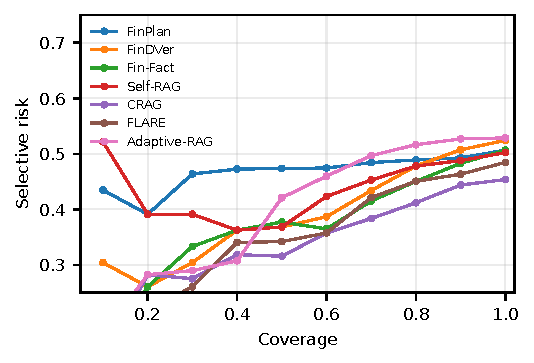
\includegraphics[width=\linewidth]{figures/risk_coverage_named.pdf}
\caption{Selective risk-coverage curves for the DeepSeek source-grounded baselines. CRAG attains the lowest AURC and the highest selective accuracy; \method{} has higher AURC but stronger balanced accuracy and AUROC.}
\label{fig:risk}
\end{figure}

\section{Sequential Evidence and Additional Results}
\label{app:sequential}

The sequential experiment uses the earliest 8-K Item 2.02 release after the cutoff. The belief model is a logistic regression on target features, peer summary features, and days since cutoff. It is trained on 2010--2020 claims, validated on 2021, and tested on the 227 verified claims from 2022--2025. The candidate policies are fixed answer, fixed adjudication, fixed abstention, always-wait, a planner without peer evidence, and a planner with peer evidence. The portfolio uses validation loss with a .1 selection margin and a .2 planner margin. The cost grid has six delay costs $\gamma\in\{0,.005,.01,.02,.05,.1\}$, two evidence costs $\{.1,.5\}$, and two outcome costs $\{2,5\}$.

Across the 24 cells, the portfolio selects always-wait in the eight cheap-delay cells and fixed adjudication in the sixteen expensive cells. Mean and maximum regret are both zero. Peer acquisition and the planner are never selected. The result depends on the earnings release, not on peer evidence: the terminal filing resolves the label, while peer outcomes are weaker than their price.

\begin{table}[t]
\centering
\small
\setlength{\tabcolsep}{3pt}
\begin{tabular}{lccc}
\toprule
Model & Acc. & Bal. & ECE \\
\midrule
\method{} (RF) & .537 & .503 & .032 \\
\method{} (logistic) & .487 & .535 & .092 \\
\bottomrule
\end{tabular}
\caption{Rolling-origin benchmark on 737 claims from 2015 to 2025.}
\label{tab:rolling}
\end{table}

The controlled diagnostic in Appendix~\ref{app:controlled} uses synthetic hidden worlds with 20 seeds and 40 cases per world. The planner reaches top-1 accuracy .899 [.886,.912], while a pre-hoc router reaches .470 [.458,.482]. The paired difference is $+.429$ [.411,.447], and all 20 seeds are positive. The diagnostic isolates the mechanism in Proposition~3: when the optimal mode depends on evidence observed after the routing decision, a pre-evidence router cannot represent the decision.

\section{Controlled Diagnostic}
\label{app:controlled}

The controlled benchmark has seven scenario families: balanced, multi-path, counterevidence-dense, sparse, source-conflict, future-revision, and random-world. Each case has a hidden state, relation templates, documents, a cutoff, a resolver, and a query budget. The planner observes the same information as the baselines and never reads hidden paths or the truth state. The preliminary signal is synthetic and its assignment is independent of pre-evidence features. The diagnostic is a mechanism test, not a financial QA result.

The planner's advantage comes from choosing the output mode after evidence. The router chooses the mode before evidence. When the optimal mode is a function of post-evidence information, the router is wrong on at least one query by construction. The empirical gap matches the proposition.

\section{Conformal Alternative}
\label{app:conformal}

We also test a conformal set constructor. LAC and APS scores form candidate sets, the threshold is selected by realized decision loss on a calibration split, and the action rule chooses among answer, set, and abstain. On the DeepSeek backbone the conformal variant reaches 3.101 at base, 1.947 under cheap abstention, 1.053 under narrow width, and 4.447 under wide width. The base value is close to the tuned fixed adjudicator (3.122) and the planner (3.119). Company masking attenuates the base advantage (3.119 versus 3.108). The conformal variant is a sensitivity analysis; the random-forest portfolio is the selected decision layer.

\end{document}
